\documentclass[aspectratio=169]{beamer}

%------------------%
% Theme & packages %
%------------------%

\usepackage{../common/beamerthemequintor}

%------------------------%
% Titelpagina informatie %
%------------------------%

\title{Performant Python Programming}
\subtitle{Van snel Python code naar snelle Python code}
\author{G.J. de Jong}
\date{02-07-2020}


%-------------------%
% Documentstructuur %
%-------------------%

\begin{document}

% Titlepage
\frame{\titlepage}

% Inhoudsopgave
\begin{frame}
  \frametitle{Inhoudsopgave}
  \tableofcontents
\end{frame}

% Python in de praktijk
\section{Python in de praktijk}
\begin{frame}
  \frametitle{Python in de praktijk}
  \begin{columns}
    \begin{column}{0.4\textwidth}
      \begin{itemize}
        \item Data science buiten de IT
        \item Veel gebruik van libraries
      \end{itemize}
    \end{column}
    \begin{column}{0.7\textwidth}
      \begin{quote}
        Professionals working with data science applications don’t want to be bogged down with complicated programming requirements.
        They want to use programming languages like Python and Ruby to perform tasks hassle-free.
      \end{quote}
    \end{column}
  \end{columns}
\end{frame}

% Performance meten
\section{Performance meten}
\begin{frame}
  \frametitle{Performance meten}
  \begin{columns}
    \begin{column}{0.5\textwidth}
      \begin{itemize}
        \item Tijd
        \item Geheugengebruik
      \end{itemize}
    \end{column}
    \begin{column}{0.5\textwidth}
    \end{column}
  \end{columns}
\end{frame}

% timeit
\subsection{timeit}
\begin{frame}[fragile]
  \frametitle{timeit}
  \begin{columns}
    \begin{column}{0.42\textwidth}
      \begin{itemize}
        \item Tool om snelheid te meten
        \item In Python Standard Library
      \end{itemize}
    \end{column}
    \begin{column}{0.68\textwidth}
      \begin{lstlisting}[language=Python, basicstyle=\small]
>>> numbers_list = list(range(9999))
>>> timeit.timeit(lambda: 5000 in numbers_list, number=1000)
0.06302383900037967
      \end{lstlisting}
      \begin{lstlisting}[language=bash, basicstyle=\small]
[denni@Arch ~]$ python -m timeit -s "numbers_list=list(range(9999))" "5000 in numbers_list"
10000 loops, best of 5: 31.2 usec per loop
      \end{lstlisting}
      \begin{lstlisting}[language=Python, basicstyle=\small]
numbers_list = list(range(9999))

%timeit 5000 in numbers_list
32.4 µs ± 310 ns per loop (mean ± std. dev. of 7 runs, 10000 loops each)
      \end{lstlisting}
    \end{column}
  \end{columns}
\end{frame}

% sys.getsizeof
\subsection{sys.getsizeof}
\begin{frame}[fragile]
  \frametitle{sys.getsizeof}
  \begin{columns}
    \begin{column}{0.42\textwidth}
      \begin{itemize}
        \item Tool om geheugengebruik te meten
        \item In Python Standard Library
      \end{itemize}
    \end{column}
    \begin{column}{0.68\textwidth}
      \begin{figure}
        \begin{lstlisting}[language=Python, basicstyle=\small]
>>> sys.getsizeof(list(range(999)))
8048
>>> sys.getsizeof(array.array('i', list(range(999))))
4060
        \end{lstlisting}
      \end{figure}
    \end{column}
  \end{columns}
\end{frame}

% Performant programmeren
\section{Performant programmeren}
\begin{frame}[fragile]
  \frametitle{Performant programmeren}
  \begin{itemize}
    \item Technieken vergelijken
  \end{itemize}
\end{frame}

% Types
\subsection{Types}
\begin{frame}[fragile]
  \frametitle{Types}
  \begin{itemize}
    \item Weet waar je mee werkt
    \item Dynamically typed
    \item Strongly typed
  \end{itemize}
  \medskip
  \begin{columns}
    \begin{column}{0.3\textwidth}
      \begin{lstlisting}[language=Python]
>>> a = 5
>>> a = str(5)
>>> a
'5'
      \end{lstlisting}
    \end{column}
    \begin{column}{0.7\textwidth}
      \begin{lstlisting}[language=Python]
>>> print("9" + 9)
Traceback (most recent call last):
File "<stdin>", line 1, in <module>
TypeError: can only concatenate str (not "int") to str
      \end{lstlisting}
    \end{column}
  \end{columns}
\end{frame}

% Data structuren
\subsection{Data structuren}
\begin{frame}[fragile]
  \frametitle{Data structuren}
  \begin{columns}
    \begin{column}{0.3\textwidth}
      \begin{itemize}
        \item List
        \item Tuple
        \item Set
        \item Dict
        \item Array
      \end{itemize}
      \medskip
      \begin{table}[]
        \begin{tabular}{llll}
              & in   & append \\
        List  & O(n) & O(1)  \\
        Tuple & O(n) &  /    \\
        Set   & O(1) & O(1)  \\
        Dict  & O(1) & O(1)  \\
        Array & O(n) & O(1)
        \end{tabular}
      \end{table}
    \end{column}
    \begin{column}{0.7\textwidth}
      \begin{lstlisting}[language=Python, basicstyle=\small]
numbers_list = list(range(9999))
numbers_tuple = tuple(range(9999))
numbers_set = set(range(9999))
numbers_dict = dict([(x, x) for x in range(9999)])
numbers_array = array.array('i', list(range(9999)))

%timeit 5000 in numbers_list
  32.4 µs ± 310 ns per loop
%timeit 5000 in numbers_tuple
  28.2 µs ± 384 ns per loop
%timeit 5000 in numbers_set
  24.2 ns ± 0.108 ns per loop
%timeit 5000 in numbers_dict
  28.3 ns ± 0.553 ns per loop
%timeit 5000 in numbers_array
  76.5 µs ± 529 ns per loop
      \end{lstlisting}
    \end{column}
  \end{columns}
\end{frame}

% Vermijd libraries
\subsection{Vermijd libraries}
\begin{frame}[fragile]
  \frametitle{Vermijd libraries}
  \begin{columns}
    \begin{column}{0.3\textwidth}
      \begin{itemize}
        \item Toegankelijkheid maakt traag
      \end{itemize}
    \end{column}
    \begin{column}{0.7\textwidth}
      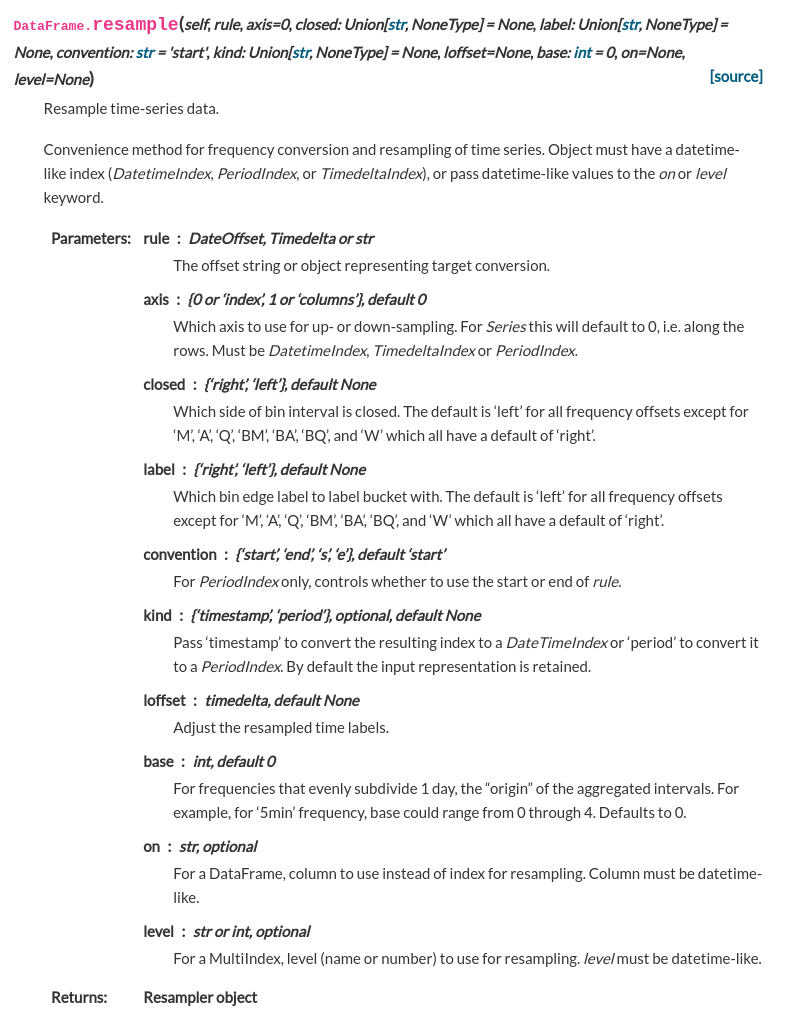
\includegraphics[height=0.95\textheight]{img/resample.png}
    \end{column}
  \end{columns}
\end{frame}

% Vermijd libraries
\begin{frame}[fragile]
  \frametitle{Vermijd libraries}
  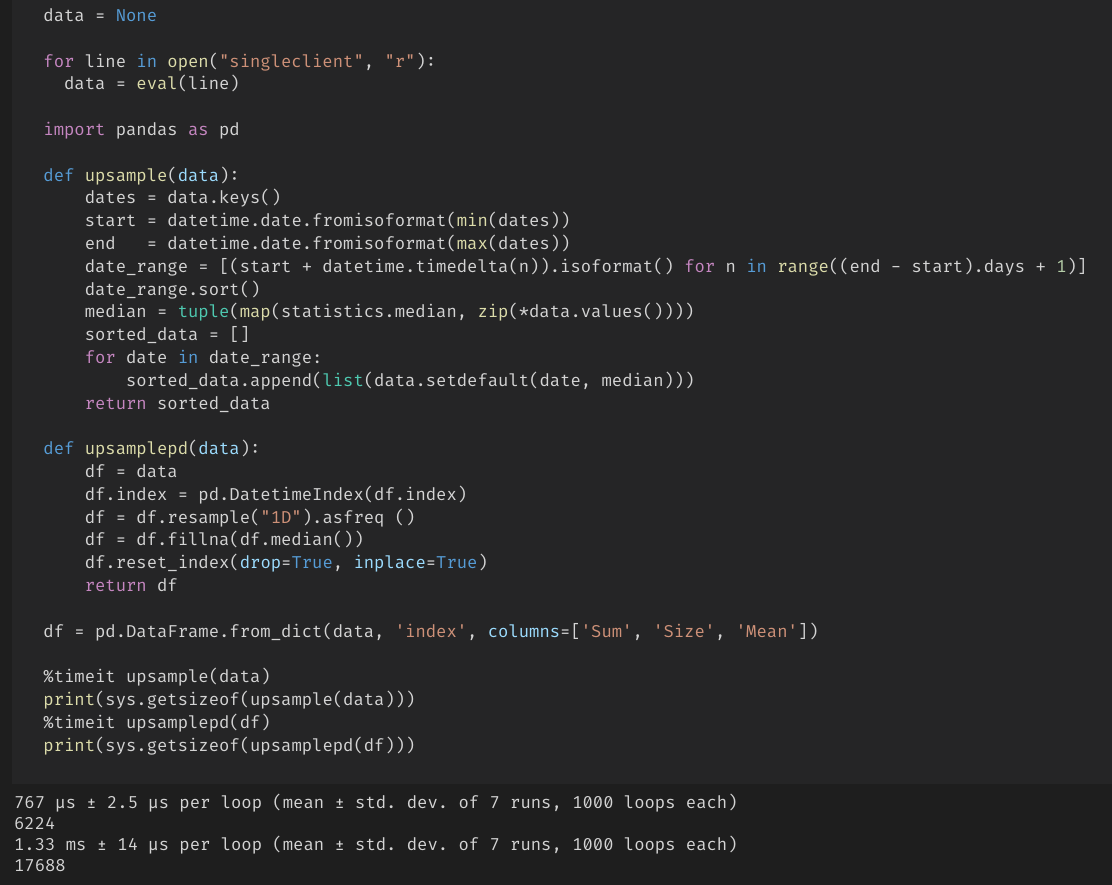
\includegraphics[height=0.95\textheight]{img/upsample.png}
\end{frame}

% Vermijd loops
\subsection{Vermijd loops}
\begin{frame}[fragile]
  \frametitle{Vermijd loops}
  \begin{columns}
    \begin{column}{0.3\textwidth}
      \begin{itemize}
        \item Loops in Python zijn niet specifiek traag
        \item Andere methodes zijn sneller
      \end{itemize}
    \end{column}
    \begin{column}{0.7\textwidth}
      \begin{lstlisting}[language=Python, basicstyle=\small]
def plusone(numbers):
  ret = []
  for n in numbers:
      ret.append(n + 1)
  return ret

numbers = range(9999)

%timeit plusone(numbers)
  487 µs ± 277 ns per loop
%timeit [n + 1 for n in numbers]
  252 µs ± 1.19 µs per loop
      \end{lstlisting}
    \end{column}
  \end{columns}
\end{frame}

% Laziness
\subsection{Laziness}
\begin{frame}[fragile]
  \frametitle{Laziness}
  \begin{columns}
    \begin{column}{0.3\textwidth}
      \begin{itemize}
        \item Developers zijn lui, waarom niet ook het programma?
      \end{itemize}
    \end{column}
    \begin{column}{0.7\textwidth}
      \begin{lstlisting}[language=Python, basicstyle=\small]
numbers = list(range(9999))

%timeit [n + 1 for n in numbers]
  250 µs ± 324 ns per loop
  87616
%timeit (n + 1 for n in numbers)
  188 ns ± 2.69 ns per loop
  112
%timeit map(lambda n: n + 1, numbers)
  142 ns ± 0.735 ns per loop
  48
      \end{lstlisting}
    \end{column}
  \end{columns}
\end{frame}

% In het kort
\section{In het kort}
\begin{frame}[fragile]
  \frametitle{In het kort}
  \begin{itemize}
    \item Weet waar je mee werkt
    \item Vermijd libraries
    \item Vermijd loops
    \item Pas laziness toe
  \end{itemize}
\end{frame}

\end{document}
